\documentclass{article}
\usepackage{CTEX}

%%%%%%%%%%%%%%%%%%%%%%%%%%%%%%%%%%%%%%%%%%%%%%%%%%%%%%%%%%%%%%%%%
\usepackage[a4paper]{geometry}
\geometry{left=3cm,right=3cm,top=3cm,bottom=3cm}
\linespread{1.5}
\usepackage{fancyhdr}

\usepackage{fontspec}
\defaultfontfeatures{Mapping=tex-text}
\usepackage{xunicode,xltxtra}
\usepackage[BoldFont,SlantFont,CJKnumber,CJKchecksingle]{xeCJK} \usepackage{CJKfntef}
\usepackage{bm} 
\usepackage{pifont}
\usepackage{color,xcolor}
\definecolor{GREEN}{RGB}{25,180,68}
\definecolor{YELLOW}{RGB}{255,255,224}
\definecolor{BLUE}{RGB}{65,105,225}
\definecolor{RED}{RGB}{139,0,0}
\definecolor{DRED}{RGB}{128,0,0}
\definecolor{GREY}{RGB}{128,128,128}

\usepackage{amsmath,amsfonts,amssymb}

\usepackage[americaninductors,europeanresistors]{circuitikz}
\usepackage{tikz}
\usetikzlibrary{positioning,arrows,shadows,shapes,calc,mindmap,trees,backgrounds}
\usepackage{graphicx}
\usepackage{subfigure} 
\usepackage{colortbl,dcolumn}  
\usepackage{multirow}
\usepackage{multicol}
\usepackage{booktabs}
\usepackage{fancyvrb}
\usepackage{listings}

\usepackage{titlesec}
\usepackage{etoolbox}
\makeatletter
\patchcmd{\ttlh@hang}{\parindent\z@}{\parindent\z@\leavevmode}{}{}
\patchcmd{\ttlh@hang}{\noindent}{}{}{}
\makeatother
\usepackage{mdwlist}
\usepackage{verbatim}
\usepackage{/Users/jinna/styles/zhfontcfg}
\usepackage{/Users/jinna/styles/visionouclistings}
\usepackage{/Users/jinna/styles/visionouccfg}
\setlength{\headheight}{15pt}
\fancyhf{}
\setCJKmainfont{Adobe Kaiti Std} 
\setCJKmonofont{Adobe Fangsong Std}
\makeatletter
\def\headrule{{\if@fancyplain\let\headrulewidth\plainheadrulewidth\fi%
\color{BLUE}
\hrule\@height 2.5pt \@width\headwidth\vskip1pt 
\hrule\@height 0.5pt\@width\headwidth              
\vskip-2\headrulewidth\vskip-1pt}        
\vspace{6mm}}                
\makeatother         

\graphicspath{{figures/}}
\tikzset{
    >=stealth',
    punkt/.style={
           rectangle,
           rounded corners,
           draw=black, very thick,
           text width=6.5em,
           minimum height=2em,
           text centered},
    pil/.style={
           ->,
           thick,
           shorten <=2pt,
           shorten >=2pt,},
    FlyZhyBall/.style={
      circle,
      minimum size=6mm,
      inner sep=0.5pt,
      ball color=red!50!blue,
      text=white,},
    FlyZhyRectangle/.style={
      rectangle,
      rounded corners,
      minimum size=6mm,
      ball color=red!50!blue,
      text=white,},
    zhyfly/.style={
      rectangle,
      rounded corners,
      minimum size=6mm,
      ball color=red!25!blue,
      text=white,},
    nrectangle/.style={
      rectangle,
      draw=#1!50,
      fill=#1!20,
      minimum size=5mm,
      inner sep=0.1pt,}
}

% code
\lstnewenvironment{VHDLcode}[1][]{%
  \lstset{
    basicstyle=\footnotesize\ttfamily\color{black},%
    columns=flexible,%
    framexleftmargin=.7mm,frame=shadowbox,%
    rulesepcolor=\color{blue},%
%    frame=single,%
    backgroundcolor=\color{yellow!20},%
    xleftmargin=1.2\fboxsep,%
    xrightmargin=.7\fboxsep,%
    numberstyle=\tiny\color{blue},%
    numberblanklines=false,numbersep=7pt,%
    language=VHDL%
    }\lstset{#1}}{}
\lstnewenvironment{VHDLmiddle}[1][]{%
  \lstset{
    basicstyle=\scriptsize\ttfamily\color{black},%
    columns=flexible,%
    framexleftmargin=.7mm,frame=shadowbox,%
    rulesepcolor=\color{blue},%
%    frame=single,%
    backgroundcolor=\color{yellow!20},%
    xleftmargin=1.2\fboxsep,%
    xrightmargin=.7\fboxsep,%
    numbers=left,numberstyle=\tiny\color{blue},%
    numberblanklines=false,numbersep=7pt,%
    language=VHDL%
    }\lstset{#1}}{}
\lstnewenvironment{VHDLsmall}[1][]{%
  \lstset{
    basicstyle=\tiny\ttfamily\color{black},%
    columns=flexible,%
    framexleftmargin=.7mm,frame=shadowbox,%
    rulesepcolor=\color{blue},%
%    frame=single,%
    backgroundcolor=\color{yellow!20},%
    xleftmargin=1.2\fboxsep,%
    xrightmargin=.7\fboxsep,%
    numbers=left,numberstyle=\tiny\color{blue},%
    numberblanklines=false,numbersep=7pt,%
    language=VHDL%
    }\lstset{#1}}{}
% pdf
\hypersetup{pdfauthor={Haiyong Zheng},%
            pdftitle={Title},%
            CJKbookmarks=true,%
            bookmarksnumbered=true,%
            bookmarksopen=false,%
            plainpages=false,%
            colorlinks=true,%
            citecolor=green,%
            filecolor=magenta,%
            linkcolor=DRED,%red(default)
            urlcolor=cyan}
\newcommand\titlebar{%
\tikz[baseline,trim left=3.1cm,trim right=3cm] {
    \fill [cyan!25] (2.5cm,-1ex) rectangle (\textwidth+3.1cm,2.5ex);
    \node [
        fill=cyan!60!white,
        anchor= base east,
        rounded rectangle,
        minimum height=3.5ex] at (3cm,0) {
        \textbf{\thesection.}
    };
}%
}

\definecolor{mygreen}{rgb}{0,0.6,0}
\definecolor{mygray}{rgb}{0.5,0.5,0.5}
\definecolor{mymauve}{rgb}{0.58,0,0.82}
\lstset{
 backgroundcolor=\color{white}, 
 basicstyle = \footnotesize,       
 breakatwhitespace = false,        
 breaklines = true,                 
 captionpos = b,                    
 commentstyle = \color{mygreen}\bfseries,
 extendedchars = false,             
 frame =shadowbox, 
 framerule=0.5pt,
 keepspaces=true,
 keywordstyle=\color{blue}\bfseries, % keyword style
 language = C++,                     % the language of code
 otherkeywords={string}, 
 numbers=left, 
 numbersep=5pt,
 numberstyle=\tiny\color{mygray},
 rulecolor=\color{black},         
 showspaces=false,  
 showstringspaces=false, 
 showtabs=false,    
 stepnumber=1,         
 stringstyle=\color{mymauve},        % string literal style
 tabsize=2,          
 title=\lstname                      
}


%%%%%%%%%%%%%%%%%%%%%%%%%%%%%%%%%%%%%%%%%%%%%%%%%%%%%%%%%%%
%设置标题页面               
\chead{\color{GREY}Experiment Report}%页眉
\cfoot{\color{GREY}12.11}%页脚 中
\lfoot{\color{GREY}Jinna}%页脚 左
\rfoot{\color{GREY}\thepage\ }%页脚 右
\renewcommand{\headrulewidth}{0.4pt}
\renewcommand{\footrulewidth}{0.4pt}
\usepackage{/Users/jinna/styles/lshort}

%%%%%%%%%%%%%%%%%%%%%%%%%%%%%%%%%%%%%%%%%%%%%%%%%%%%%%%%%%%%%%%%%
\begin{document}

\pagenumbering{roman}


\pagestyle{fancy}
%%%%%%%%%%%%%%%%%%%%%%%%%%%%%%%%%%%%%%%%%%%%%%%%%%%%%%%%%%%%%%%%%
\begin{center}
\textbf{\LARGE{Experiment Report}} %标题加黑加大居
\end{center}

\begin{center}
Jinna Cui
\end{center}

\begin{center}
12.19 - 12.25
\end{center}


I have used Gaussian low-pass filtering to get the global features of images. With this method, both the texture and shape are blurred. In fact, we want to get clear shape information with weak texture information. Gaussian low-pass filter can weaken texture information but also weaken the shape information because clear boundaries become blurred after Gaussian low-pass filter. In response to this difficulty, I tried bilateral filter algorithm, which has the role of edge-preserving and denoising. The result shows that bilateral filter works better than Gaussian low-pass filter. With bilateral filter, we can get clear boundaries and shape information while the texture information is effectively weakened. 
\begin{figure}[!ht] 
  \centering 
  \subfigure[original image]{ 
    \label{fig:subfig:a} %% label for first subfigure 
    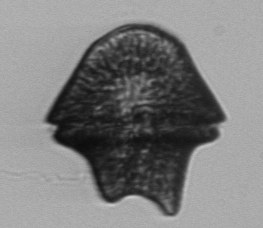
\includegraphics[width=4cm,height=3cm]{1.png}} 
  \hspace{0.3in} 
  \subfigure[Gaussian low-pass filter image]{ 
    \label{fig:subfig:b} %% label for second subfigure 
    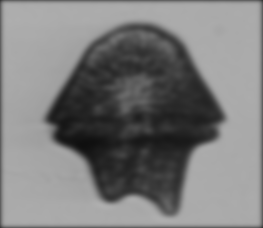
\includegraphics[width=4cm,height=3cm]{5.png}} 
   \hspace{0.3in} 
   \subfigure[Image after once bilateral filter ]{ 
    \label{fig:subfig:b} %% label for second subfigure 
    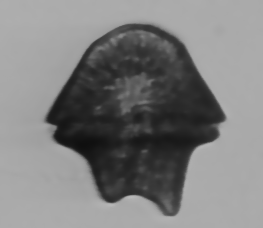
\includegraphics[width=4cm,height=3cm]{2.png}} 
   \hspace{0.3in} 
   \subfigure[Image after three times bilateral filter]{ 
    \label{fig:subfig:b} %% label for second subfigure 
    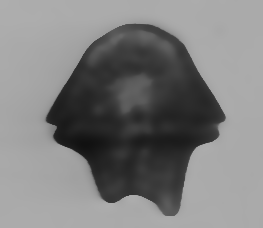
\includegraphics[width=4cm,height=3cm]{3.png}} 
   \hspace{0.3in} 
   \subfigure[Image after ten times bilateral filter ]{ 
    \label{fig:subfig:b} %% label for second subfigure 
    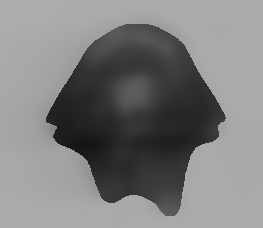
\includegraphics[width=4cm,height=3cm]{4.png}} 
   \hspace{0.3in}  
  \label{fig:subfig} %% label for entire figure 
\end{figure}

The filter effect is showed in above pictures. As we can see, with multiple times bilateral filter  details are weakened and the boundary is more clearly. More filtering leads to better results. Unluckily, bilateral filter costs too much time. So, I decide to process images with bilateral filter for three times.  In this way, most textures are weakened and costs less time. 

As the bilateral filter costs too much time, the filtering speed is about 800 - 5000 images per hour (it depends on whether the computer is busy or not). So the whole WHOI-Plankton database which contains 3.6 millions images is impossible for me. As a result, I picked the images collected in 2013 about 410 thousands images out as training database and pick images collected in 2014 about 320 thousands images out as test database. But the amount is still huge. As this database contains 103 classes images, one class named `mix' consists of all unidentified images. Mix classes contains about 300 thousands images in training database and about 240 thousands images in test database. So I deleted this class. And there are 4 classes in training database are empty but in test database is not empty. So I also delete these four classes: Akashiwo, DIdinium-sp, Kiteflagellates, Leptocylidrus\_mediterraneus. In this way, I got a training database with about 110 thousands images and a test database with about 60 thousands images. In total, there are 98 classes. With this 98 classes database, I got a benchmark on AlexNet. The accuracy is 87.51\%. Now I am try to process the `mix' class images by bilateral filter. This may cost about ten days(both mix in train database and test database and processed by the server and my Mac). 

Next week, I will mainly focus on the three-channel work and do more experiments on caffe. Besides, I want to try to abstract local features and global features by neural network. Last days, I read a paper named \textbf{Extraction of Skin Lesions from Non-Dermoscopic Images Using Deep Learning} \url{https://arxiv.org/pdf/1609.02374v1.pdf}. Maybe I can try this kind of methods to abstract local and global features.

\end{document}